

\begin{frame}
    \frametitle{Stolpci in slike}
\end{frame}



\begin{frame}{Konstrukcija pravokotnice na premico $p$ skozi točko $T$}

		\begin{columns}
		\column{0.55\textwidth}
		\begin{itemize}[<+->]
            \item<1-> Dani sta premica $p$ in točka $T$. 
            \item<2-> Nariši lok $k$ s središčem v $T$. 
            \item<3-> Premico $p$ seče v točkah $A$ in $B$. 
            \item<4-> Nariši lok $m$ s središčem v $A$. 
            \item<5-> Nariši lok $n$ s središčem v $B$ in z enakim polmerom. 
            \item<6-> Loka se sečeta v točki $C$. 
            \item<7> Premica skozi točki $T$ in $C$ je pravokotna na $p$. 
        \end{itemize}
		\column{0.45\textwidth}
		\only<1>{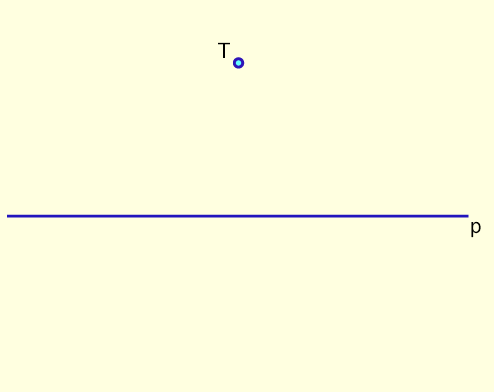
\includegraphics[width=\textwidth]{prosojnice/fig-1.png}}
        \only<2>{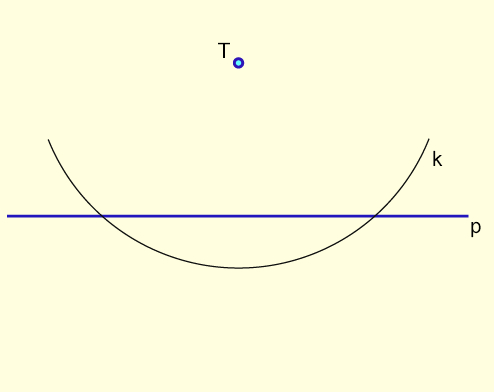
\includegraphics[width=\textwidth]{prosojnice/fig-2.png}}
        \only<3>{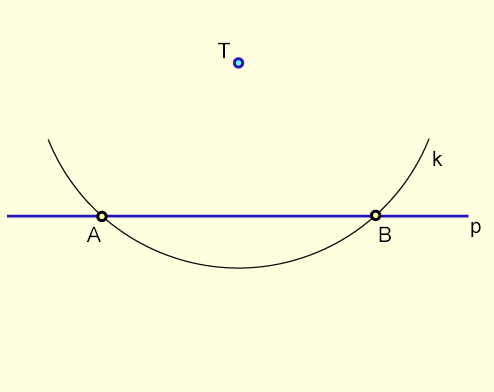
\includegraphics[width=\textwidth]{prosojnice/fig-3.png}}
        \only<4>{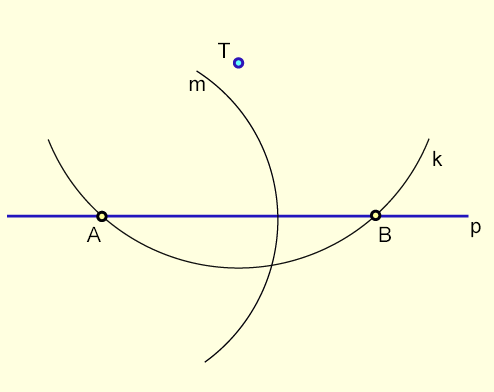
\includegraphics[width=\textwidth]{prosojnice/fig-4.png}}
        \only<5>{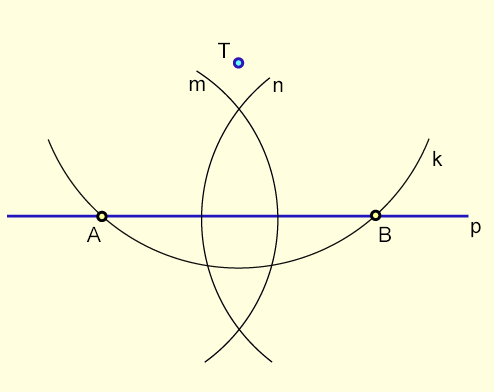
\includegraphics[width=\textwidth]{prosojnice/fig-5.png}}
        \only<6>{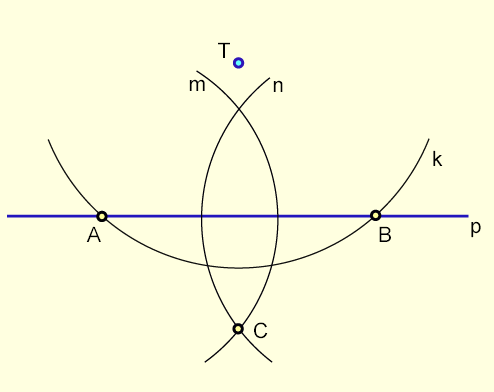
\includegraphics[width=\textwidth]{prosojnice/fig-6.png}}
        \only<7>{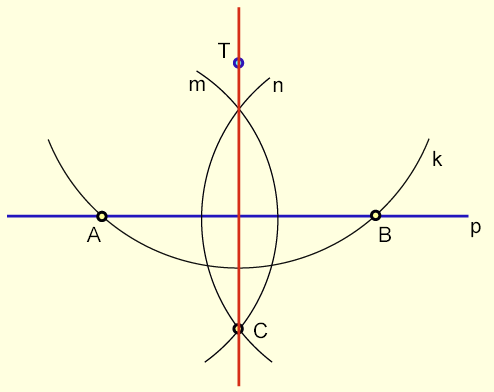
\includegraphics[width=\textwidth]{prosojnice/fig-7.png}}
		\end{columns}

    \end{frame}

	\begin{frame}{Konstrukcija pravokotnice na premico $p$ skozi točko $T$}

		\begin{columns}
			\column{0.55\textwidth}
			\begin{itemize}[<+->]
				\item Dani sta premica $p$ in točka $T$.
				\item Nariši lok $k$ s središčem v $T$.
				\item Premico $p$ seče v točkah $A$ in $B$.
				\item Nariši lok $m$ s središčem v $A$.
				\item Nariši lok $n$ s središčem v $B$ in z enakim polmerom.
				\item Loka se sečeta v točki $C$.
				\item Premica skozi točki $T$ in $C$ je pravokotna na $p$.
			\end{itemize}
			\column{0.45\textwidth}
			
			\begin{tikzpicture}[scale=1.2]
					\tikzmath{
						\t = 2*sin(45);
						\tt = 2*sin(60);
						\td = \t - 2*cos(60);
					}
					
					% Točka T
					\coordinate [label={[blue, above left]:$T$}] (T) at (0,{\t});
					\fill[blue] (T) circle (2pt);
					
					% Premica p
					\draw[blue, very thick] (-2,0) -- (2,0) node[right] {$p$};
				
					% 1. Lok k (središče v T, preseka p v A in B)
					\onslide<2->{ 
						\coordinate (A') at ({-\tt},{\td});
						\draw[gray, thin] (A') arc[start angle=210, end angle=330, radius=2] node[right] {\scriptsize $k$};
					}
				
					% 2. Točka A
					\onslide<3->{
						\coordinate [label=below left:{\scriptsize $A$}] (A) at ({-\t},0);
						\fill (A) circle (1.5pt);
						\coordinate [label=below left:{\scriptsize $B$}] (B) at ({\t},0);
						\fill (B) circle (1.5pt);	
					}
					\onslide<4->{
						\coordinate (D) at ({-\td},{\tt}); 
						\draw[gray, thin] (D) arc[start angle=60, end angle=-60, radius=2] node[left] {\scriptsize $m$};
					}
					\onslide<5->{
						\coordinate (S) at ({\td},{\tt}); 
						\draw[gray, thin] (S) arc[start angle=120, end angle=240, radius=2] node[right] {\scriptsize $n$};
					}
					\onslide<6->{\coordinate [label=below:{\scriptsize $C$}] (C) at (0,{-\t});
					\fill (C) circle (1.5pt);
						
					}
					\onslide<7>{\draw[red, thick] (0,-2) -- (0,2);
					}
				\end{tikzpicture}
		\end{columns}
	
	\end{frame}

				
 %Naloga 4
 \begin{frame}{Graf funkcije s TikZ}
	\centering
	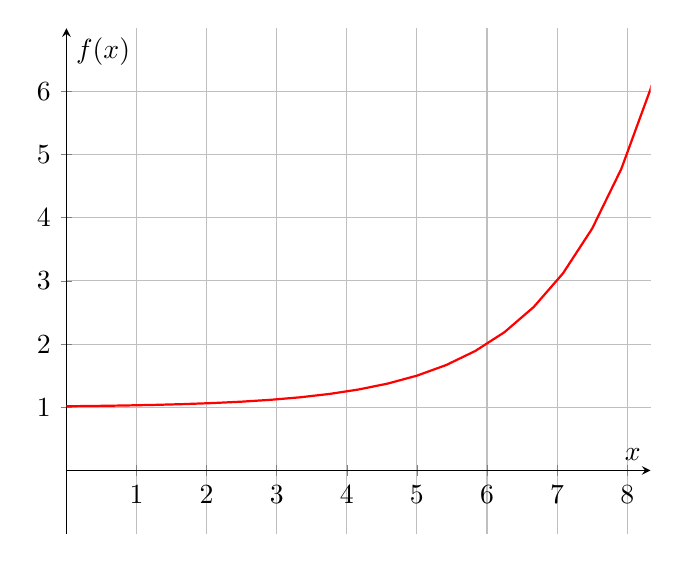
\begin{tikzpicture}
		\begin{axis}[
		   axis lines = middle,
			domain = 0:10,
			height = 8cm,
		   width = 9cm,
		   xtick = {0, 1, 2, 3, 4, 5, 6, 7, 8},
			ytick = {0, 1, 2, 3, 4, 5, 6},
			ymin = -1,
			ymax = 7,
			grid = both,
		   xlabel = {\(x\)},
		   ylabel = {\(f(x)\)}
		]
	   \addplot[color=red, thick]{2^(x-6) + 1};
		\end{axis}
	\end{tikzpicture}
\end{frame}
